\documentclass{standalone}
\usepackage{tikz}
\usetikzlibrary{patterns, positioning}


\begin{document}
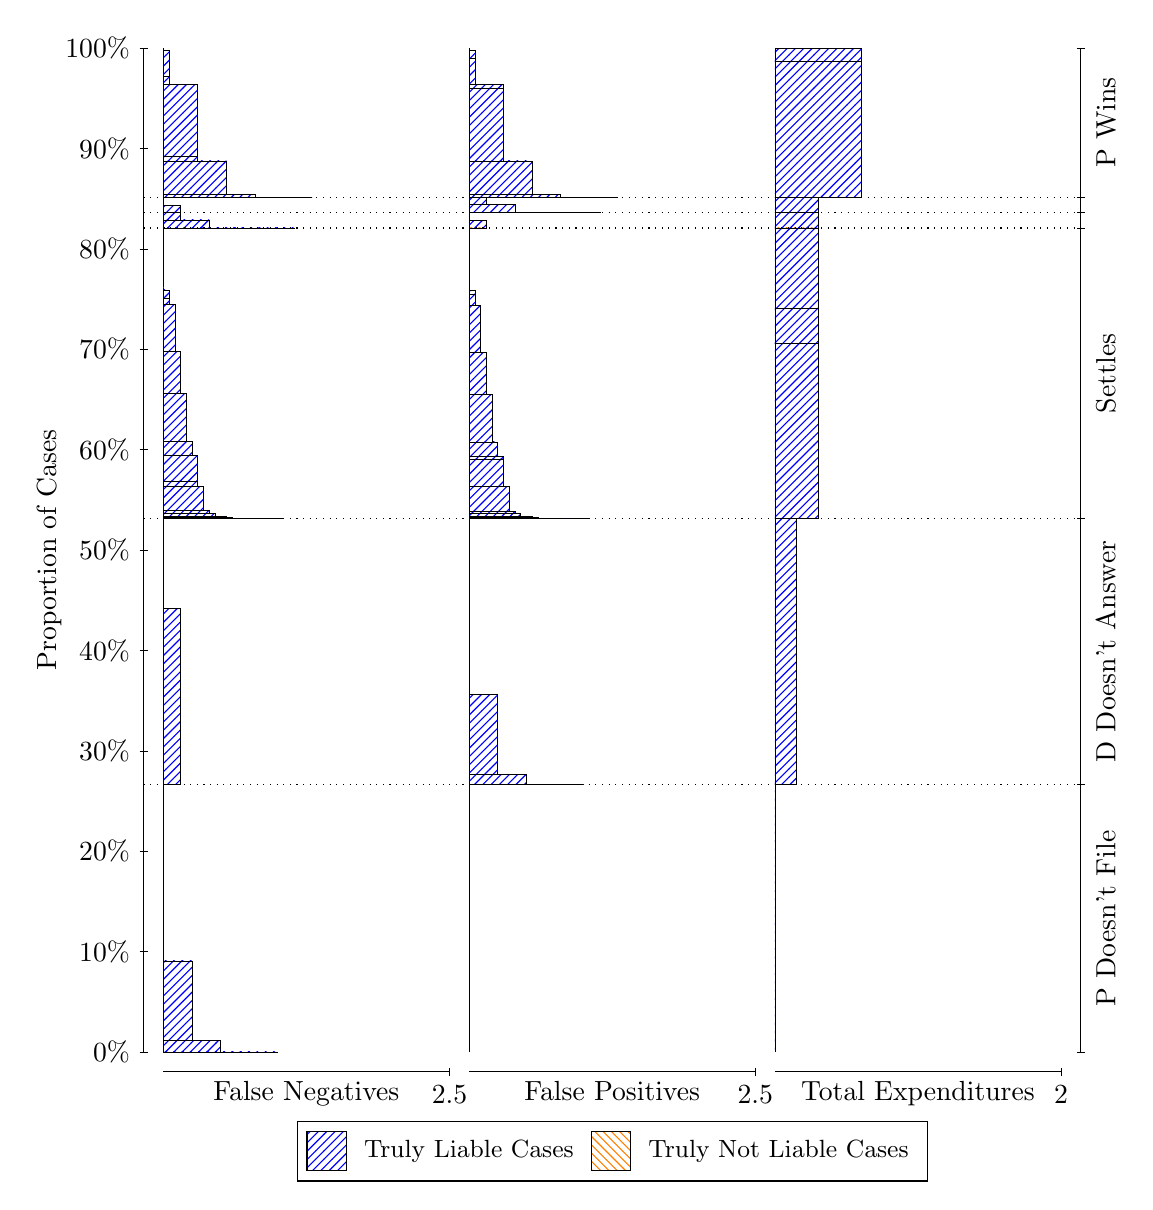
\begin{tikzpicture}
\draw[black, very thin] (1.5,1.75) -- (1.5,14.5);
\node[rotate=90, text=black, anchor=center] at (0.3, 8.125) {Proportion of Cases};
\draw[black, very thin] (1.45,1.75) -- (1.55,1.75);
\node[text=black, anchor=east] at (1.45, 1.75) {0\%};
\draw[black, very thin] (1.45,3.025) -- (1.55,3.025);
\node[text=black, anchor=east] at (1.45, 3.025) {10\%};
\draw[black, very thin] (1.45,4.3) -- (1.55,4.3);
\node[text=black, anchor=east] at (1.45, 4.3) {20\%};
\draw[black, very thin] (1.45,5.575) -- (1.55,5.575);
\node[text=black, anchor=east] at (1.45, 5.575) {30\%};
\draw[black, very thin] (1.45,6.85) -- (1.55,6.85);
\node[text=black, anchor=east] at (1.45, 6.85) {40\%};
\draw[black, very thin] (1.45,8.125) -- (1.55,8.125);
\node[text=black, anchor=east] at (1.45, 8.125) {50\%};
\draw[black, very thin] (1.45,9.4) -- (1.55,9.4);
\node[text=black, anchor=east] at (1.45, 9.4) {60\%};
\draw[black, very thin] (1.45,10.675) -- (1.55,10.675);
\node[text=black, anchor=east] at (1.45, 10.675) {70\%};
\draw[black, very thin] (1.45,11.95) -- (1.55,11.95);
\node[text=black, anchor=east] at (1.45, 11.95) {80\%};
\draw[black, very thin] (1.45,13.225) -- (1.55,13.225);
\node[text=black, anchor=east] at (1.45, 13.225) {90\%};
\draw[black, very thin] (1.45,14.5) -- (1.55,14.5);
\node[text=black, anchor=east] at (1.45, 14.5) {100\%};

\draw[black, very thin] (13.4,1.75) -- (13.4,14.5);
\draw[black, very thin] (13.35,1.75) -- (13.45,1.75);
\node[anchor=west] at (13.35, 1.75) {};
\draw[black, very thin] (13.35,5.1439) -- (13.45,5.1439);
\node[anchor=west] at (13.35, 5.1439) {};
\draw[black, very thin] (13.35,8.5262) -- (13.45,8.5262);
\node[anchor=west] at (13.35, 8.5262) {};
\draw[black, very thin] (13.35,12.215) -- (13.45,12.215);
\node[anchor=west] at (13.35, 12.215) {};
\draw[black, very thin] (13.35,12.411) -- (13.45,12.411);
\node[anchor=west] at (13.35, 12.411) {};
\draw[black, very thin] (13.35,12.606) -- (13.45,12.606);
\node[anchor=west] at (13.35, 12.606) {};
\draw[black, very thin] (13.35,14.5) -- (13.45,14.5);
\node[anchor=west] at (13.35, 14.5) {};

\draw[black, very thin, pattern color=blue, pattern=north east lines] (1.75,1.75) rectangle (3.2033,1.75);
\draw[black, very thin, pattern color=blue, pattern=north east lines] (1.75,1.75) rectangle (2.84,1.7512);
\draw[black, very thin, pattern color=blue, pattern=north east lines] (1.75,1.7512) rectangle (2.4767,1.8952);
\draw[black, very thin, pattern color=blue, pattern=north east lines] (1.75,1.8952) rectangle (2.1133,2.9077);
\draw[black, very thin, pattern color=orange, pattern=north west lines] (1.75,2.9077) rectangle (1.75,2.9077);
\draw[black, very thin, pattern color=blue, pattern=north east lines] (1.75,2.9077) rectangle (1.75,5.1439);
\draw[black, very thin, pattern color=blue, pattern=north east lines] (1.75,5.1439) rectangle (1.968,7.3806);
\draw[black, very thin, pattern color=orange, pattern=north west lines] (1.75,7.3806) rectangle (1.75,7.3806);
\draw[black, very thin, pattern color=blue, pattern=north east lines] (1.75,7.3806) rectangle (1.75,8.5262);
\draw[black, very thin, pattern color=blue, pattern=north east lines] (1.75,8.5262) rectangle (3.276,8.5262);
\draw[black, very thin, pattern color=blue, pattern=north east lines] (1.75,8.5262) rectangle (2.9853,8.5262);
\draw[black, very thin, pattern color=blue, pattern=north east lines] (1.75,8.5262) rectangle (2.9127,8.5262);
\draw[black, very thin, pattern color=blue, pattern=north east lines] (1.75,8.5262) rectangle (2.84,8.5262);
\draw[black, very thin, pattern color=blue, pattern=north east lines] (1.75,8.5262) rectangle (2.6947,8.5262);
\draw[black, very thin, pattern color=blue, pattern=north east lines] (1.75,8.5262) rectangle (2.622,8.5345);
\draw[black, very thin, pattern color=blue, pattern=north east lines] (1.75,8.5345) rectangle (2.5493,8.5524);
\draw[black, very thin, pattern color=blue, pattern=north east lines] (1.75,8.5524) rectangle (2.4767,8.553);
\draw[black, very thin, pattern color=blue, pattern=north east lines] (1.75,8.553) rectangle (2.404,8.5878);
\draw[black, very thin, pattern color=blue, pattern=north east lines] (1.75,8.5878) rectangle (2.3313,8.6232);
\draw[black, very thin, pattern color=blue, pattern=north east lines] (1.75,8.6232) rectangle (2.2587,8.9328);
\draw[black, very thin, pattern color=blue, pattern=north east lines] (1.75,8.9328) rectangle (2.186,9.0023);
\draw[black, very thin, pattern color=blue, pattern=north east lines] (1.75,9.0023) rectangle (2.186,9.3233);
\draw[black, very thin, pattern color=blue, pattern=north east lines] (1.75,9.3233) rectangle (2.1133,9.5068);
\draw[black, very thin, pattern color=blue, pattern=north east lines] (1.75,9.5068) rectangle (2.0407,10.112);
\draw[black, very thin, pattern color=blue, pattern=north east lines] (1.75,10.112) rectangle (1.968,10.644);
\draw[black, very thin, pattern color=blue, pattern=north east lines] (1.75,10.644) rectangle (1.8953,11.244);
\draw[black, very thin, pattern color=blue, pattern=north east lines] (1.75,11.244) rectangle (1.8227,11.324);
\draw[black, very thin, pattern color=blue, pattern=north east lines] (1.75,11.324) rectangle (1.8227,11.429);
\draw[black, very thin, pattern color=blue, pattern=north east lines] (1.75,11.429) rectangle (1.75,11.459);
\draw[black, very thin, pattern color=orange, pattern=north west lines] (1.75,11.459) rectangle (1.75,11.459);
\draw[black, very thin, pattern color=blue, pattern=north east lines] (1.75,11.459) rectangle (1.75,12.215);
\draw[black, very thin, pattern color=blue, pattern=north east lines] (1.75,12.215) rectangle (3.4213,12.215);
\draw[black, very thin, pattern color=blue, pattern=north east lines] (1.75,12.215) rectangle (3.058,12.215);
\draw[black, very thin, pattern color=blue, pattern=north east lines] (1.75,12.215) rectangle (2.6947,12.217);
\draw[black, very thin, pattern color=blue, pattern=north east lines] (1.75,12.217) rectangle (2.3313,12.316);
\draw[black, very thin, pattern color=blue, pattern=north east lines] (1.75,12.316) rectangle (1.968,12.411);
\draw[black, very thin, pattern color=orange, pattern=north west lines] (1.75,12.411) rectangle (1.75,12.411);
\draw[black, very thin, pattern color=blue, pattern=north east lines] (1.75,12.411) rectangle (1.968,12.505);
\draw[black, very thin, pattern color=orange, pattern=north west lines] (1.75,12.505) rectangle (1.75,12.505);
\draw[black, very thin, pattern color=blue, pattern=north east lines] (1.75,12.505) rectangle (1.75,12.606);
\draw[black, very thin, pattern color=blue, pattern=north east lines] (1.75,12.606) rectangle (3.6393,12.606);
\draw[black, very thin, pattern color=blue, pattern=north east lines] (1.75,12.606) rectangle (3.276,12.606);
\draw[black, very thin, pattern color=blue, pattern=north east lines] (1.75,12.606) rectangle (2.9127,12.639);
\draw[black, very thin, pattern color=blue, pattern=north east lines] (1.75,12.639) rectangle (2.5493,13.066);
\draw[black, very thin, pattern color=blue, pattern=north east lines] (1.75,13.066) rectangle (2.186,13.119);
\draw[black, very thin, pattern color=blue, pattern=north east lines] (1.75,13.119) rectangle (2.186,14.04);
\draw[black, very thin, pattern color=blue, pattern=north east lines] (1.75,14.04) rectangle (1.8227,14.135);
\draw[black, very thin, pattern color=blue, pattern=north east lines] (1.75,14.135) rectangle (1.8227,14.467);
\draw[black, very thin, pattern color=orange, pattern=north west lines] (1.75,14.467) rectangle (1.75,14.467);
\draw[black, very thin, pattern color=blue, pattern=north east lines] (1.75,14.467) rectangle (1.75,14.5);
\draw[black, very thin, pattern color=orange, pattern=north west lines] (5.6333,1.75) rectangle (5.6333,1.75);
\draw[black, very thin, pattern color=blue, pattern=north east lines] (5.6333,1.75) rectangle (5.6333,5.1439);
\draw[black, very thin, pattern color=orange, pattern=north west lines] (5.6333,5.1439) rectangle (7.0867,5.1439);
\draw[black, very thin, pattern color=blue, pattern=north east lines] (5.6333,5.1439) rectangle (7.0867,5.1439);
\draw[black, very thin, pattern color=blue, pattern=north east lines] (5.6333,5.1439) rectangle (6.7233,5.1445);
\draw[black, very thin, pattern color=blue, pattern=north east lines] (5.6333,5.1445) rectangle (6.36,5.2757);
\draw[black, very thin, pattern color=blue, pattern=north east lines] (5.6333,5.2757) rectangle (5.9967,6.2895);
\draw[black, very thin, pattern color=blue, pattern=north east lines] (5.6333,6.2895) rectangle (5.6333,8.5262);
\draw[black, very thin, pattern color=orange, pattern=north west lines] (5.6333,8.5262) rectangle (7.1593,8.5262);
\draw[black, very thin, pattern color=blue, pattern=north east lines] (5.6333,8.5262) rectangle (7.1593,8.5262);
\draw[black, very thin, pattern color=orange, pattern=north west lines] (5.6333,8.5262) rectangle (6.8687,8.5262);
\draw[black, very thin, pattern color=blue, pattern=north east lines] (5.6333,8.5262) rectangle (6.8687,8.5262);
\draw[black, very thin, pattern color=blue, pattern=north east lines] (5.6333,8.5262) rectangle (6.796,8.5262);
\draw[black, very thin, pattern color=orange, pattern=north west lines] (5.6333,8.5262) rectangle (6.7233,8.5262);
\draw[black, very thin, pattern color=blue, pattern=north east lines] (5.6333,8.5262) rectangle (6.7233,8.5262);
\draw[black, very thin, pattern color=orange, pattern=north west lines] (5.6333,8.5262) rectangle (6.578,8.5262);
\draw[black, very thin, pattern color=blue, pattern=north east lines] (5.6333,8.5262) rectangle (6.578,8.5262);
\draw[black, very thin, pattern color=blue, pattern=north east lines] (5.6333,8.5262) rectangle (6.5053,8.5344);
\draw[black, very thin, pattern color=orange, pattern=north west lines] (5.6333,8.5344) rectangle (6.4327,8.5344);
\draw[black, very thin, pattern color=blue, pattern=north east lines] (5.6333,8.5344) rectangle (6.4327,8.5519);
\draw[black, very thin, pattern color=orange, pattern=north west lines] (5.6333,8.5519) rectangle (6.4327,8.5519);
\draw[black, very thin, pattern color=blue, pattern=north east lines] (5.6333,8.5519) rectangle (6.4327,8.552);
\draw[black, very thin, pattern color=blue, pattern=north east lines] (5.6333,8.552) rectangle (6.36,8.5525);
\draw[black, very thin, pattern color=orange, pattern=north west lines] (5.6333,8.5525) rectangle (6.2873,8.5525);
\draw[black, very thin, pattern color=blue, pattern=north east lines] (5.6333,8.5525) rectangle (6.2873,8.5871);
\draw[black, very thin, pattern color=blue, pattern=north east lines] (5.6333,8.5871) rectangle (6.2147,8.6194);
\draw[black, very thin, pattern color=blue, pattern=north east lines] (5.6333,8.6194) rectangle (6.142,8.9283);
\draw[black, very thin, pattern color=blue, pattern=north east lines] (5.6333,8.9283) rectangle (6.0693,9.2823);
\draw[black, very thin, pattern color=blue, pattern=north east lines] (5.6333,9.2823) rectangle (6.0693,9.3125);
\draw[black, very thin, pattern color=orange, pattern=north west lines] (5.6333,9.3125) rectangle (5.9967,9.3125);
\draw[black, very thin, pattern color=blue, pattern=north east lines] (5.6333,9.3125) rectangle (5.9967,9.4969);
\draw[black, very thin, pattern color=blue, pattern=north east lines] (5.6333,9.4969) rectangle (5.924,10.098);
\draw[black, very thin, pattern color=blue, pattern=north east lines] (5.6333,10.098) rectangle (5.8513,10.63);
\draw[black, very thin, pattern color=blue, pattern=north east lines] (5.6333,10.63) rectangle (5.7787,11.235);
\draw[black, very thin, pattern color=blue, pattern=north east lines] (5.6333,11.235) rectangle (5.706,11.378);
\draw[black, very thin, pattern color=blue, pattern=north east lines] (5.6333,11.378) rectangle (5.706,11.418);
\draw[black, very thin, pattern color=blue, pattern=north east lines] (5.6333,11.418) rectangle (5.6333,12.215);
\draw[black, very thin, pattern color=orange, pattern=north west lines] (5.6333,12.215) rectangle (5.8513,12.215);
\draw[black, very thin, pattern color=blue, pattern=north east lines] (5.6333,12.215) rectangle (5.8513,12.31);
\draw[black, very thin, pattern color=blue, pattern=north east lines] (5.6333,12.31) rectangle (5.6333,12.411);
\draw[black, very thin, pattern color=orange, pattern=north west lines] (5.6333,12.411) rectangle (7.3047,12.411);
\draw[black, very thin, pattern color=blue, pattern=north east lines] (5.6333,12.411) rectangle (7.3047,12.411);
\draw[black, very thin, pattern color=blue, pattern=north east lines] (5.6333,12.411) rectangle (6.9413,12.411);
\draw[black, very thin, pattern color=blue, pattern=north east lines] (5.6333,12.411) rectangle (6.578,12.413);
\draw[black, very thin, pattern color=blue, pattern=north east lines] (5.6333,12.413) rectangle (6.2147,12.512);
\draw[black, very thin, pattern color=blue, pattern=north east lines] (5.6333,12.512) rectangle (5.8513,12.606);
\draw[black, very thin, pattern color=orange, pattern=north west lines] (5.6333,12.606) rectangle (7.5227,12.606);
\draw[black, very thin, pattern color=blue, pattern=north east lines] (5.6333,12.606) rectangle (7.5227,12.606);
\draw[black, very thin, pattern color=orange, pattern=north west lines] (5.6333,12.606) rectangle (7.1593,12.606);
\draw[black, very thin, pattern color=blue, pattern=north east lines] (5.6333,12.606) rectangle (7.1593,12.606);
\draw[black, very thin, pattern color=orange, pattern=north west lines] (5.6333,12.606) rectangle (6.796,12.606);
\draw[black, very thin, pattern color=blue, pattern=north east lines] (5.6333,12.606) rectangle (6.796,12.639);
\draw[black, very thin, pattern color=orange, pattern=north west lines] (5.6333,12.639) rectangle (6.4327,12.639);
\draw[black, very thin, pattern color=blue, pattern=north east lines] (5.6333,12.639) rectangle (6.4327,13.066);
\draw[black, very thin, pattern color=blue, pattern=north east lines] (5.6333,13.066) rectangle (6.0693,13.987);
\draw[black, very thin, pattern color=orange, pattern=north west lines] (5.6333,13.987) rectangle (6.0693,13.987);
\draw[black, very thin, pattern color=blue, pattern=north east lines] (5.6333,13.987) rectangle (6.0693,14.04);
\draw[black, very thin, pattern color=blue, pattern=north east lines] (5.6333,14.04) rectangle (5.706,14.372);
\draw[black, very thin, pattern color=blue, pattern=north east lines] (5.6333,14.372) rectangle (5.706,14.468);
\draw[black, very thin, pattern color=blue, pattern=north east lines] (5.6333,14.468) rectangle (5.6333,14.5);
\draw[black, very thin, pattern color=orange, pattern=north west lines] (9.5167,1.75) rectangle (9.5167,1.75);
\draw[black, very thin, pattern color=blue, pattern=north east lines] (9.5167,1.75) rectangle (9.5167,5.1439);
\draw[black, very thin, pattern color=orange, pattern=north west lines] (9.5167,5.1439) rectangle (9.7892,5.1439);
\draw[black, very thin, pattern color=blue, pattern=north east lines] (9.5167,5.1439) rectangle (9.7892,8.5262);
\draw[black, very thin, pattern color=orange, pattern=north west lines] (9.5167,8.5262) rectangle (10.062,8.5262);
\draw[black, very thin, pattern color=blue, pattern=north east lines] (9.5167,8.5262) rectangle (10.062,10.747);
\draw[black, very thin, pattern color=orange, pattern=north west lines] (9.5167,10.747) rectangle (10.062,10.747);
\draw[black, very thin, pattern color=blue, pattern=north east lines] (9.5167,10.747) rectangle (10.062,11.191);
\draw[black, very thin, pattern color=orange, pattern=north west lines] (9.5167,11.191) rectangle (10.062,11.191);
\draw[black, very thin, pattern color=blue, pattern=north east lines] (9.5167,11.191) rectangle (10.062,12.215);
\draw[black, very thin, pattern color=orange, pattern=north west lines] (9.5167,12.215) rectangle (10.062,12.215);
\draw[black, very thin, pattern color=blue, pattern=north east lines] (9.5167,12.215) rectangle (10.062,12.411);
\draw[black, very thin, pattern color=orange, pattern=north west lines] (9.5167,12.411) rectangle (10.062,12.411);
\draw[black, very thin, pattern color=blue, pattern=north east lines] (9.5167,12.411) rectangle (10.062,12.606);
\draw[black, very thin, pattern color=orange, pattern=north west lines] (9.5167,12.606) rectangle (10.607,12.606);
\draw[black, very thin, pattern color=blue, pattern=north east lines] (9.5167,12.606) rectangle (10.607,14.331);
\draw[black, very thin, pattern color=orange, pattern=north west lines] (9.5167,14.331) rectangle (10.607,14.331);
\draw[black, very thin, pattern color=blue, pattern=north east lines] (9.5167,14.331) rectangle (10.607,14.5);
\draw[black, dotted] (1.5,5.1439) -- (13.4,5.1439);
\draw[black, dotted] (1.5,8.5262) -- (13.4,8.5262);
\draw[black, dotted] (1.5,12.215) -- (13.4,12.215);
\draw[black, dotted] (1.5,12.411) -- (13.4,12.411);
\draw[black, dotted] (1.5,12.606) -- (13.4,12.606);
\draw[black, very thin] (1.75,1.5) -- (5.3833,1.5);
\node[text=black, anchor=north] at (3.5667, 1.5) {False Negatives};
\draw[black, very thin] (5.3833,1.45) -- (5.3833,1.55);
\node[text=black, anchor=north] at (5.3833, 1.45) {2.5};

\draw[black, very thin] (5.6333,1.5) -- (9.2667,1.5);
\node[text=black, anchor=north] at (7.45, 1.5) {False Positives};
\draw[black, very thin] (9.2667,1.45) -- (9.2667,1.55);
\node[text=black, anchor=north] at (9.2667, 1.45) {2.5};

\draw[black, very thin] (9.5167,1.5) -- (13.15,1.5);
\node[text=black, anchor=north] at (11.333, 1.5) {Total Expenditures};
\draw[black, very thin] (13.15,1.45) -- (13.15,1.55);
\node[text=black, anchor=north] at (13.15, 1.45) {2};

\node[text=black, centered, rotate=90] at (13.72, 3.447) {P Doesn't File};
\node[text=black, centered, rotate=90] at (13.72, 6.8351) {D Doesn't Answer};
\node[text=black, centered, rotate=90] at (13.72, 10.371) {Settles};


\node[text=black, centered, rotate=90] at (13.72, 13.553) {P Wins};

\draw (7.449999999999999,1.5) node[draw=none] (baseCoordinate) {};
\begin{scope}[align=center]
        \matrix[scale=0.5, draw=black, below=0.5cm of baseCoordinate, nodes={draw}, column sep=0.1cm]{
            \node[rectangle, draw, minimum width=0.5cm, minimum height=0.5cm, pattern color=blue, pattern=north east lines] {}; &
            \node[draw=none, font=\small, text=black] (B) {Truly Liable Cases}; &
            \node[rectangle, draw, minimum width=0.5cm, minimum height=0.5cm, pattern color=orange, pattern=north west lines] {}; &
            \node[draw=none, font=\small, text=black] (B) {Truly Not Liable Cases}; \\
            };
\end{scope}

\end{tikzpicture}
\end{document}